%%%%%%%%%%%%%%%%%%%%%%%%%%%%%%%%%%%%%%%%%
% Homework Assignment Article
% LaTeX Template
% Version 1.3.1 (ECL) (08/08/17)
%
% This template has been downloaded from:
% Overleaf
%
% Original author:
% Victor Zimmermann (zimmermann@cl.uni-heidelberg.de)
%
% License:
% CC BY-SA 4.0 (https://creativecommons.org/licenses/by-sa/4.0/)
%
%%%%%%%%%%%%%%%%%%%%%%%%%%%%%%%%%%%%%%%%%

%----------------------------------------------------------------------------------------

\documentclass[a4paper]{article} % Uses article class in A4 format

%----------------------------------------------------------------------------------------
%	FORMATTING
%----------------------------------------------------------------------------------------

\addtolength{\hoffset}{-2.25cm}
\addtolength{\textwidth}{4.5cm}
\addtolength{\voffset}{-3.25cm}
\addtolength{\textheight}{5cm}
\setlength{\parskip}{0pt}
\setlength{\parindent}{0in}

%----------------------------------------------------------------------------------------
%	PACKAGES AND OTHER DOCUMENT CONFIGURATIONS
%----------------------------------------------------------------------------------------

\usepackage{blindtext} % Package to generate dummy text
% \usepackage[style=numeric,sorting=none]{biblatex}
\usepackage{charter} % Use the Charter font
\usepackage[utf8]{inputenc} % Use UTF-8 encoding
\usepackage{microtype} % Slightly tweak font spacing for aesthetics

\usepackage[english]{babel} % Language hyphenation and typographical rules

\usepackage{amsthm, amsmath, amssymb} % Mathematical typesetting
\usepackage{float} % Improved interface for floating objects
\usepackage[final, colorlinks = true, 
            linkcolor = black, 
            citecolor = black]{hyperref} % For hyperlinks in the PDF
\usepackage{graphicx, multicol} % Enhanced support for graphics
\usepackage{xcolor} % Driver-independent color extensions
\usepackage{marvosym, wasysym} % More symbols
\usepackage{rotating} % Rotation tools
\usepackage{censor} % Facilities for controlling restricted text
\usepackage{listings, style/lstlisting} % Environment for non-formatted code, !uses style file!
\usepackage{pseudocode} % Environment for specifying algorithms in a natural way
\usepackage{style/avm} % Environment for f-structures, !uses style file!
\usepackage{booktabs} % Enhances quality of tables

\usepackage{tikz-qtree} % Easy tree drawing tool
\tikzset{every tree node/.style={align=center,anchor=north},
         level distance=2cm} % Configuration for q-trees
\usepackage{style/btree} % Configuration for b-trees and b+-trees, !uses style file!

% \usepackage[backend=biber,style=numeric,
            % sorting=nyt]{biblatex} % Complete reimplementation of bibliographic facilities
% \addbibresource{ecl.bib}
\usepackage{csquotes} % Context sensitive quotation facilities

\usepackage[yyyymmdd]{datetime} % Uses YEAR-MONTH-DAY format for dates
\renewcommand{\dateseparator}{-} % Sets dateseparator to '-'

\usepackage{fancyhdr} % Headers and footers
\pagestyle{fancy} % All pages have headers and footers
\fancyhead{}\renewcommand{\headrulewidth}{0pt} % Blank out the default header
\fancyfoot[L]{School of Computing, Macquarie University} % Custom footer text
\fancyfoot[C]{} % Custom footer text
\fancyfoot[R]{\thepage} % Custom footer text
\graphicspath{{./images/}}

\usepackage{comment}
\newcommand{\note}[1]{\marginpar{\scriptsize \textcolor{red}{#1}}} % Enables comments in red on margin

%----------------------------------------------------------------------------------------

\begin{document}

%----------------------------------------------------------------------------------------
%	TITLE SECTION
%----------------------------------------------------------------------------------------

\title{COMP3100 project report} % Article title
\fancyhead[C]{}
\hrule \medskip % Upper rule
\begin{minipage}{1\textwidth} % Center of title section
\centering 
\large % Title text size
Project report: Stage 1\\ % Assignment title and number
COMP3100 Distributed Systems, S1, 2023\\
\normalsize % Subtitle text size
SID\@: 46598634, Name: Justin Bedwany\\
Github repository link: \url{https://github.com/jbedwany/COMP3100-Assignment}
%%%%\\ % Assignment subtitle
\end{minipage}
\medskip\hrule % Lower rule
\bigskip

%----------------------------------------------------------------------------------------
%	ARTICLE CONTENTS
%----------------------------------------------------------------------------------------
\section{Introduction} % 1/2 page
%Brief introduction of your stage~\cite{mesos2011}.
This project is the creation of a client using the Java programming language for participation in a simulated distributed computing system. The client connects to a provided distributed systems job server, receives 
information about the available participating servers, then is issued jobs for which it must choose an appropriate server with which the job is then scheduled. The client will utilise the Largest-Round-Robin (LRR) format 
for scheduling jobs, where the `largest' (i.e.\ highest number of cores) type of participant server is identified, then each available server of that type is issued a job in a round-robin fashion.\\

This project forms Stage 1 of a larger project. The overall goal of both stages is to develop a functional client which implements multiple scheduling algorithms, to be compared with a number of baseline algorithms 
such as First Fit,  Best Fit, and Worst Fit. In Stage 1, the primary goal is to develop the baseline client which successfully connects to the \texttt{ds-sim} server provided 
\href{https://github.com/distsys-MQ/ds-sim}{here} [], correctly parses server information, and schedules jobs identically to the reference \texttt{ds-sim} client (when operating in LRR mode). 

\section{System Overview} % 1/2 page
The client interacts with the \texttt{ds-sim} server. The interaction can be summarised by 3 stages: \\
\begin{enumerate}
    \item Connection \& Preamble
    \item Job Generation \& Scheduling
    \item Termination
\end{enumerate}
The below diagram indicates each step of the process. Connection, Authentication, and Parsing Server Info form Stage 1, the loop between Receive Job and Schedule Job form Stage 2, and Quit If None Available forms Stage 3.
\begin{figure}[h]
    \centering
    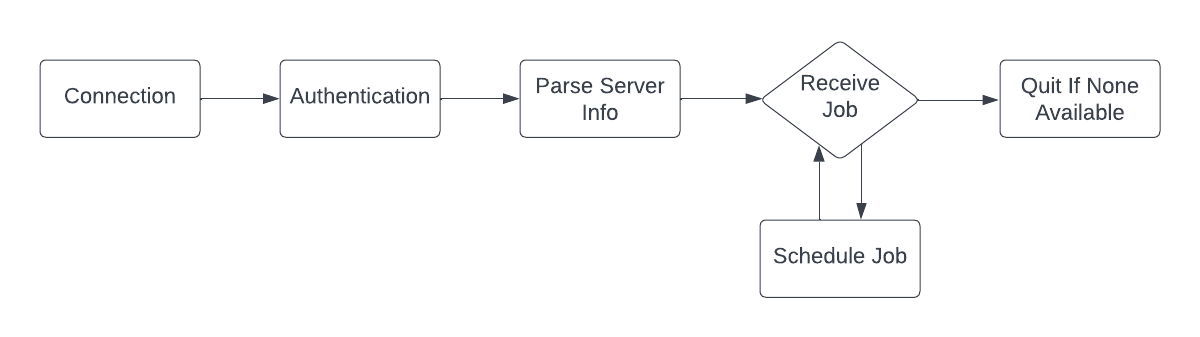
\includegraphics[width=\textwidth]{Workflow.png}
    \caption{Process Outline}
\end{figure}\\
The jobs generated and scheduled are entirely independent of each other --- i.e.\ no job depends on another job being completed first. Due to the guarantee within the specification that no job will require more resources 
than those of the largest server type, no capability checking is performed prior to issuing each job to each server.

\pagebreak
\section{Design} % 1 page
%design philosophy, considerations and constraints, functionalities of each simulator component focusing on the client-side simulator
\subsection{Philosophy}
The major aspect of design philosophy is a focus on simplicity for users and in code architecture. Aside from a number of runtime arguments, namely the server host address, the port, and the user to authenticate as, the 
person running the simulation does not need to interact with the client for it to function. Programmatically, the code developed utilises the DRY (Don't Repeat Yourself) principle by compartmentalising and reusing code 
where appropriate in order to improve comprehension and maintenance.
\subsection{Considerations, Limitations, \& Assumptions}
Future readability and ease of extension has been the chief consideration in this project, as it forms Stage 1 of a two stage project, and will therefore be built upon in future. Documentation is being created alongside 
the project in order to facilitate consistency in direction as well as ensure minimal operating details are lost.\\
The project is limited in that it currently only uses the LRR format for scheduling jobs; whenever any other format is required, this implementation of the client will not be suitable. Additionally, jobs are not scheduled 
in parallel --- any given server that may be able to handle multiple jobs simultaneously are only ever given one at a time.\\
It has been assumed that no jobs generated require more resources than those of the largest server provided. This is a condition on which the \texttt{ds-sim} server operates and therefore will always be true for the 
purposes of each simulation, but must be considered when drawing real-world conclusions from simulation data.
\subsection{Server Simulator}
The server simulator functions by reading a configuration file which defines properties of servers and jobs that will be dynamically generated. Once the client connects and completes the preamble, the server will generate 
a job to be scheduled or information regarding the job queue or server statuses. This will repeat for the duration of the simulation.
\subsection{Client Simulator}
The client simulator functions by connecting to the server simulator, receiving information about the available servers, then receiving information about the current job to be scheduled. It then makes a scheduling decision 
based on the available servers and their capacities. Afterwards, it requests a new job to process, and the cycle repeats until the server responds with `NONE', indicating there are no more jobs to be completed. The simulation 
then ends.

\begin{figure}[h]
    \centering
    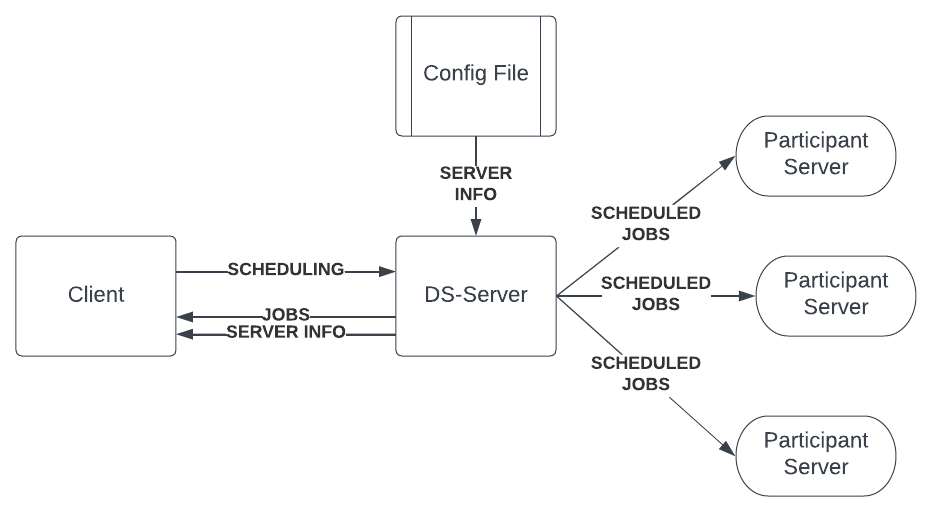
\includegraphics[height=8cm]{System Structure.png}
    \caption{System Structure}
\end{figure}

\pagebreak
\section{Implementation} % 2 pages
A number of key decisions have been made as part of this implementation. Structurally, the code is separated into the following sections:
\begin{enumerate}
    \item Input Validation
    \item Connection to Server
    \item Identification of Largest Server Type
    \item Scheduling of Job
    \item Connection Termination
    \item Helper Functions
\end{enumerate}
It also makes use of two custom-defined classes, Job and Server. 
\subsection{Object-Oriented Programming}
Java is an Object-Oriented Programming language, which means it is designed to handle complex data structures through the definition of classes\ \cite{javadoc}. This is relevant for this project, because each job and server 
provided by the \texttt{ds-sim} server contains multiple data fields, and in the case of the servers, multiple data types (strings e.g.\ server type and integers e.g.\ server ID). There are a number of ways to handle this, 
such as multi-dimensional arrays (e.g.\ one dimension for each job, and one dimension for each field within each job), however being a strongly typed language, arrays containing multiple datatypes are not possible --- which 
is an issue for keeping track of the servers involved.\\
Instead, by defining a class each for Job and Server, we can cleanly unite all the relevant fields within a single object for both jobs and servers, and we get a bonus of being able to include as a built-in function of 
those objects for parsing the strings received from the \texttt{ds-sim} server declaring each job or server. This allows us to keep the main program clean and easy to read, both through modularisation of code functions 
as well as simplifying data structures in use, but also provides scalability options --- for example, when implementing an alternative method for determining which server to schedule which job on, a comparison function can 
be trivially included within the job or server class definition to allow comparing jobs requirements with server capabilities.

\subsection{Job Scheduling}
The client schedules jobs based on a Largest Round-Robin format. After connecting to the \texttt{ds-sim} server, it retrieves the list of available servers using the \texttt{GETS All} command. It parses the results of this 
command in order to determine the available servers, and identifies the largest server based on the amount of cores each has. The provided server list does not need to be sorted in order of server size to accurately 
determine the largest server type. After the largest server type is identified, it creates a list of them, then as each JOBN command is received from the \texttt{ds-sim} server, it iterates through this list with each 
server having a turn completing a job, then repeats from the start. This continues until the \texttt{ds-sim} server issues the \texttt{NONE} command, indicating there are no jobs left to be processed. 
It then terminates the connection.

\subsection{Helper Functions}
A number of helper functions have been created in order to keep the main logic of the program clean and easy to read. As message sending and receiving is done in the same way repeatedly throughout the program, including 
message logging, they have been converted into functions.\\
As the methodology of finding the largest server is somewhat cumbersome, it has been separated into its own helper function. First, it issues and receives the data. It uses array data structures throughout instead of 
ArrayLists, which have convenient built-in functionality of being able to be resized (as compared to Arrays which cannot be, and must have new arrays of the correct size redeclared). This would have been used to potentially 
simply remove the elements of the servers list that were not needed (i.e.\ not of the largest type) and retain the same data structure, thereby reducing overhead. However, the implementation of ArrayLists is such that 
appending an element to the list is done by creating a new array of the correct size and moving the elements across with the new element at the end. As numerous elements are added to the array iteratively, it is therefore 
much more efficient to simply create a new array containing only the largest servers.

% brief description of any implementation specific information including technologies, techniques, software libraries and data structures used. How each of components/functions
% of your simulator is implemented
% talk about job and server objects & OOP in general


%----------------------------------------------------------------------------------------
%	REFERENCE LIST
%----------------------------------------------------------------------------------------
\bibliographystyle{ieeetr}
\bibliography{comp3100project}
%----------------------------------------------------------------------------------------
\end{document}